% this file is called up by thesis.tex
% content in this file will be fed into the main document

%: ----------------------- name of chapter  -------------------------
\chapter{Analiza problemu integracji systemów przetwarzania mowy} % top level followed by section, subsection


%: ----------------------- paths to graphics ------------------------

% change according to folder and file names
\ifpdf
    \graphicspath{{2/figures/PNG/}{2/figures/PDF/}{2/figures/}}
\else
    \graphicspath{{2/figures/EPS/}{2/figures/}}
\fi

%: ----------------------- contents from here ------------------------

Rozdział ten podzielony jest na trzy części. Celem pierwszej jest zdefiniowanie pojęcia przetwarzania mowy, celem drugiej jest analiza różnych, możliwych sposobów integracji natomiast celem częsci trzeciej jest opisanie jak specyficzna dziedzina, jaką jest przetwarzanie mowy, wpływa na wybór sposobu integracji.

\section{Przetwarzanie mowy}
Mowa jest naturalnym, wybranym przez człowieka w procesie ewolucji, sposobem komunikacji. Jej niewątpliwe zalety to:
\begin{itemize}
	\item brak konieczności stosowania sprzętu
	\item komunikacja mimo braku fizycznego kontaktu
	\item nie istnienie potrzeby widzenia rozmówcy
	\item umożliwianie komunikacji w czasie wykonywania innych czynności
\end{itemize}
Wraz z rozwojem cywylizacyjnym ewoluował także sposób komunikacji i jej format. Najpierw zaczęto mowę spisywać ręcznie, następnie stworzono maszyny drukarskie, aż w końcu zaczęto stosować do tego celu zapis cyfrowy i komputery. Użycie tych ostatnich umożliwia nie tylko przechowywanie mowy ale także jej przetwarzanie. Pod tym pojęciem może kryć się wiele różnych procesów. Najważniejsze oraz najczęsciej stosowane z nich to:
\begin{itemize}
	\item rozpoznawanie mowy, często oznaczane skrótem ASR ( z języka angielskiego automatic speech recognition)
	\item synteza mowy, oznaczane jako TTS ( z języka angielskiego Text To Speech)
	\item optyczne rozpoznawanie tekstu (tekst można traktować jako zapis mowy), oznaczane skrótem OCR (z języka angielskiego Optical Character Recognition)
	\item tłumaczenie mowy
	\item rozpoznawanie języka
\end{itemize} 
\subsection{Rozpoznawanie mowy}
Rozpoznawanie mowy jest to technologia umożliwiająca komputerowi wyposażonemu w odpowiednie urządzenie na przykład mikrofon interpretować ludzką mowę i zamieniać ją na tekst \cite{douglas2002}. Systemy oferujące przetwarzanie mowy można rozróżniać	 według dwóch różnych kryteriów:
\begin{itemize}
	\item sposobu uczenia się
	\item sposobu rozpoznawania mowy
\end{itemize}
Stosując pierwsze kryterium, aplikacje można podzielić na
\begin{itemize}
	\item zależne od lektora
	\item niezależne od lektora
\end{itemize}
Systemy należące do pierwszej grupy uczą się poprzez sesje w czasie których lektor czyta porcje tekstu, aplikacje analizują głos, ton oraz tępo  w efekcie czego mogą dostosować się do danego lektora co skutkuje uzyskują uzyskaniem o wiele dokładniejszych wyników, w przedziale 95-100\%, oczywiście przy założeniu, że lektor ma podobny głos.  Systemy należące do drugiej grupy uczy się przy wykorzystaniu różnych lektorów. Uzyskiwane przez nie wyniki rzadko przekracają 75% jednak są dużo bardziej stabilne, to znaczy nie zależnie od lektora wyniki są w tej okolicy. 
Stosując kryterium drugie wyrózniamy następujące grupy systemów \cite{gaikwad2010} :
\begin{itemize}
	\item Rozpoznające izolowane słowa - są to dość proste systemy, posiadające dwa stany: nasłuchujący i nie nasłuchujący,  wymagające ciszy na początku i na końcu każdej wypowiedzi,  akceptują jedno słowo lub krótką wypowiedź 
	\item Rozpoznające łączone słowa - podobne do systemów z grupy powyżej, charakteryzują się znacznie większą czułoscią na przerwy pomiędzy kolejnymi słowami czyli umożliwiają osobnym wypowiedziom występować tylko, z minimalnymi przerwami pomiędzy nimi
	\item Rozpoznające mowę ciągłą -  systemy z tej grupy umożliwiają użytkownikowi mówienie w sposób niemal naturalny w czasie gdy one rozpoznają zawartość. Są to najnowsze i najbardziej zaawansowane systemy.
\end{itemize}
\subsection{Synteza mowy}   
Synteza mowy jest sztuczną produkcją ludzkiej mowy. Syntezatory, czyli systemy komputerowe, które dokonują syntezy można podzielić na grupy stosując dwa różne kryteria:
\begin{itemize}
	\item sposób implementacji
	\item sposób tworzenia mowy
\end{itemize}
Systemy należące do pierwszej grupy można podzielić na:
\begin{itemize}
	\item implementowane programowo
	\item implementowane sprzętowo
\end{itemize}
Kategoria pierwsza jest bardziej liczna, łatwiej dostępna, tańsza przez co też dużo bardziej popularna. Dużą zaletą aplikacji należących do pierwszej grupy jest ich uniwersalność,  mogą one być łatwo wykorzystani do różnych celów takich jak:
\begin{itemize}
	\item lektorzy filmowi/e-książek/emaili
	\item poczty głosowe
	\item pomoc techniczna
	\item interaktywnej obsługi osoby  dzwoniącej
\end{itemize}
Najpopularniejsze syntezatory mowy dostępne na rynku to:
\begin{itemize}
	\item IvonaTTS
	\item TextAloud
	\item Loquendo
\end{itemize}
Systemy należące do kategorii drugiej (implementowane sprzętowo) charakteryzują się dużo większą wydajnością i szybkością działania. Najlepsze z nich są w stanie generować mowę w czasie rzeczywistym. 
Ze względu na sposób tworzenia mowy, systemy można podzielić na:
\begin{itemize}
	\item Syntezatory artykulacyjne stosują metodę polegającą na kontrolowaniu artykulatorów mowy takich jak szczęka, język, policzki itd. Systemy te próbują modelować mechaniczne ruchy artykulatorów.
	\item Syntezatory korzystające z metody konkatenacyjnej korzystają z dużej bazy oznaczonych próbek(słów) prawdziwego głosu lektora, proces syntezy sprowadza się do wybranie, modyfikacji i konkatenacji tych nagrań. 
	\item Syntezatory alofoniczne, w czasie działania składają potrzebne słowa z dźwięków elementarnych przechowywanych w pamięci i wywoływanych w odpowiedniej chwili. 
\end{itemize}
\subsection{Optyczne rozpoznawanie tekstu}
Optyczne rozpoznawanie tekstu, dużo częściej występujące w wersji skróconej OCR, to mechaniczna lub elektroniczna konwersja obrazu pisma ręcznego, maszynowego lub wydrukowanego tekstu do postacicyfrowej pozwalającej na dalszą jego obróbkę. Podobnie jak w przypadku syntezatorów mowy systemy OCR można podzielić na:
\begin{itemize}
	\item implementowane programowo
	\item implementowane sprzętowo
\end{itemize}
Podobnie jak przy syntezatorach zaletą implementacji sprzętowej jest szybkość oraz wydajność co umożliwia pracę w czasie rzeczywistym. Niezależnie od implementacji, sposyb ich działania oraz algorytmy pozostają podobne. Podstawowe kroki jakie system musi podjąc w celu rozpoznania tekstu to \cite{noor2005} :
\begin{enumerate}
	\item Wczytanie obrazu jako mapy bitowej z podanego źródła.
	\item Rozpoznanie najważniejszych cech obrazu takich jak rozdzielczość i inwersja. Wiele algorytmów spodziewa się kolorów i rozmiaru czcionki w ramach predefiniowanego przedziału dlatego też obraz musi być przeskalowany i znormalizowany przed dalszą obróbką. Na tym etapie rozpoznawane również są pozycje i typy najważniejszych części obrazu.
	\item Wiele algorytmów wymaga by obraz był dwu kolorowy, dlatego kolorowy albo szary obraz musi być przekonwertowany do biało czarnej postaci, to bardzo istotny krok algorytmu ponieważ błędy w tej części mogą powodować poważne problemy w dalszych etapach.
	\item Kolejnym ważnym krokiem jest usunięcię wszystkich podkreśleń, obramowań itd. w dalszej kolejności umożliwia to rozpoznanie linii tekstu co jest jednym z kluczowych kroków poprawnego algorytmu.
	\item Po podzieleniu tekstu na linie, algorytm stara się rozpoznać błedne znaki, to znaczy takie które stykają się z innymi albo są podzielone na kilka części (np. w wyniku konwersji do bialo czarnej postaci), i je dopasować do znanej mu puli.
	\item Ostatnim i najważniejszym krokiem jest rozpoznanie pojedynczych znaków, sukces tego kroku zależy od poprzednich etapów. Najpierw każdemu znakowi próbuje się dopasować kod znaku, czasami nie jest możliwe dopasowanie tylko jednego kodu, np. w przypadku litery \textbf{I} większość algorytmów rozpona ją jako \textbf{I}, \textbf{|}, \textbf{1} lub \textbf{i}. W takim przypadku należy skorzystać ze słownika, posiadanie bogatej bazy słów, może, w sposób znaczący poprawić efektywność algorytmu.
\end{enumerate}
Nie jest to kompletna lista kroków, istnieje dużo innych mniejszych lub większych etapów, jednak każdy z wymienionych jest bardzo ważny, cały proces nie zakończy się sukcesem jeżeli zawiedzie którykolwiek z nich. 
\subsection{Translacja mowy}
Translacja mowy to tłumaczenie z jednego języka na inny. Aplikacje tłumaczące często nazywane są translatorami. Mimo, że z pozoru mogłoby się wydawać, że jest to czynność prostsza niż OCR czy też ASR to tak nie jest. Proces tłumaczenia jest bardzo trudny i do tej pory nie istnieją aplikacje nie popełniające błedów. W zasadzie można wyróżnić trzy typy translatorów, bazując na algorytmach jakie stosują co do tłumaczonego tekstu:
\begin{itemize}
	\item algorytmy oparte na zasadach gramatyki
	\item algorytmy bazujące na podejściu statystycznym
	\item algorytmy stosujące translacje opartą o przykłady
\end{itemize}
W podejściu pierwszym przeprowadza się tłumaczenie bazując na informacjach językowych na temat języka źródłowego i docelowego. Algorytm rozkłada zdanie na części pierwsze, analizuje je, następnie bazując na bazie wiedzy którą posiada, a w skład której wchodzą informacje na temat składni, budowy zdań, odmian oraz słownik dwujęzyczny, buduje zdanie w języku docelowym. Technika ta wymaga ogromnej mocy obliczeniowej oraz dużych zasobów danych, według ekspertów w dziedzinie translacji, takich jak Franz Josef Och, jest nieefektywna.
W podejściu statystycznym tłumaczenia dokonuje się w oparciu o statystyczny model którego parametry są wyliczane na podstawie analizy tekstu. Jest do podejście mające bardzo mocne oparcie w teorii informacji. W chwili obecnej wydaje się, że jest ono najbardziej efektywne o czym może świadczyć fakt, że podejście to zostało zastosowane przez Google'a przy tworzeniu Google Translator, który wygrał międzynarodowe zawody w tłumaczeniu z angielskiego na arabski i angielskiego na chiński.
Stosowanie algorytmów opartych o analogie jest najprostszym z możliwych podejść, może być postrzegane jako implementacja uczenia maszynowego w podejściu CBR \footnote{http://www.ai-cbr.org/classroom/cbr-review.html}. Uważa się, że podejście to najbardziej dokładnie oddaje proces myślowy człowieka tłumaczącego tekst, to znaczy najpierw następuje dekompozycja zdania na mniejsze frazy, następnie tłumaczy się te frazy pojedynczo i odpowiedno łączy tworząc zdanie w języku docelowym. Traslator bazujący na takim podejściu musi przejść fazę uczenia, polegającą na podawaniu na wejście podobnych zdań w dwóch językach różniących się tylko nieznacznie. Stosując dwa proste zdania w językach angielski i japońskim: 
 \begin{itemize}
	\item ang: \verb"How much is that red umbrella?" jap: \verb"Ano akai kasa wa ikura desu ka?"
	\item ang: \verb"How much is that small camera?" jap: \verb"Ano chiisai kamera wa ikura desu ka?"
\end{itemize} 
system nauczy się, że:
 \begin{enumerate}
	\item \verb"How much is X?" odpowiada \verb"Ano X wa ikura desu ka?"
	\item \verb"red umbrella" odpowiada \verb"akai kasa"
	\item \verb"small camera" odpowiada \verb"chiisai kamera"
\end{enumerate} 
Następnie aplikacja może zastosować w ten sposób nabytą wiedzę w bardziej zaawansowanych przypadkach.
\subsection{Rozpoznawanie języka}
Rozpoznawanie języka to proces którego celem jest stwierdzenie w jakim języku naturalnym jest podany na wejście tekst \cite{adams1997} . Tradycyjne podejście, stosowane np. w księgarniach, opiera się na ręcznym zidentyfikowaniu najczęściej występujących słów i liter które są charakterystyczne dla danego języka i sprawdzenie ich w odpowiednich tabelach. Implementacja algorytmów działących na podobnej zasadzie jest możliwa jednak jest to rozwiązanie mało efektywne. Obecnie stosuje się kilka różnych podejść bazujących na statystyce:
 \begin{itemize}
	\item Bardzo prostą techniką jest porównywanie jakości kompresji badanego tekstu z jakością kompresji tekstów w znanych językach, im bardziej zbliżone wyniki tym większe prawdopodobieństwo, że teksty są w tym samym języku. Podejście to nazywa się miarą odległości wzajemnej informacji.
	\item Bardziej zaawansowanym algorytmem jest ten zaproponowany przez W.Cavnar'a i J.Trenkle'a w 1994 roku pod nazwą: "N-Gram-Based Text Categorization". Najpierw należy utworzyć znakowy n-gramowy model języka na podstawie materiałów treningowych dla każdego z języków które mają być obsługiwane. Następnie dla każdego tekstu którego język ma być zidentyfikowany, tworzy się podobny model i porównuje z modelami bazowymi. Im bardziej są do siebie podobne tym więszka szansa, że to ten sam język. Problematyczne w tym podejściu są języki dla których nie można skonstruować takiego modelu. 
	\item Rozszerzeniem poprzedniego algorytmu jest technika zaproponowa przez Panów Rehurek i Kolkus \cite{rehurek2009} . Największymi zaletami ulepszonej wersji jest fakt, że nie zawodzi ona w sytuacji w której próbka tekstu jest napisana w wielu językach, a także nie stanowi dla niej problemu rozróżnianie języków należących do tej samej rodziny (np. polski i słowacki). 
\end{itemize} 
Jak widać przetwarzanie mowy samo w sobie jest bardzo obszernym i skomplikowanym tematem, w skład którego wchodzi wiele różnych procesów które można zintegrować tworząc efektywne i bardzo funkcjonalne systemy.


\section{Sposoby integracji}
Dzięki postępowi technologicznemu przepustowość łączy internetowych wciąż wzrasta, dzięki temu to co pare lat temu było nie osiągalne dzis jest normą. Powstają nowe rodzaje usług, które kiedyś nie mogły by zostać zrealizowane, przy tworzeniu zaś niektórych aplikacji, to co kiedyś było problemem i na czym skupiali swój wysiłek twórcy oprogramowania, dzisiaj schodzi na drugi plan. Z drugiej jednak strony zwiększają sie wymagania użytkowników co do jakości, są wprowadzane coraz to nowe formaty, które wymagają ogromnych przepustowość. Czasami jednak systemy nie mają takich scisłych wymagań co do wielkości opóźnienia. W ich przypadku opóźnienie nawet rzędu kilkudziesięciu sekund nie stanowi problemu i jest akceptowalne przez użytkowników. W takim wypadku nie trzeba sie skupiać na szukaniu idealnego rozwiązania dla danego problemu, lecz można skupić się na stworzeniu architektóry która ułatwi i przyspieszy budowanie systemów spełniających dane wymagania.

Przy takim podejściu do tworzenia systemu zazwyczaj pojawia sie problem integracji budowanego systemu z istniejącymi już usługami. Często też, budowany system jest całkowicie problemem integracyjnym, czyli wszystkie składowe usługi potrzebne do realizacji celu biznesowego są dostępne, a jedyne zadanie stawiane budowanemu systemowi to opdowiednia integracja tych usług. Podejście takie ułatwia parę kwesti, ale w zamian wprowadza także nowe, specyficzne dla siebie problemy. Głownym problememe jest różnorodność dostępnych podsystemów. Każdy z nich może być stworzony przy użyciu innych technologii (Java, COM, .Net, CORBA, ICE, itp.) działać na innej platformie (MS WINDOWS, LINUX, SOLARIS) i co najważniejsze mogą wykorzystywać inne protokoły do komunikacji (RPC, SOAP, własnościowe protokoły, itp). Z tego powodu decyzja o sposobie integracji nie może byc podejmowana zbyt szybko,  powinna być podjęta bazując na pewnych kryteriach:  \cite{hohpewoolf2003} 

\begin{itemize}
	\item \textbf{powiązanie aplikacji} - integracja aplikacji powinna minimalizować powiązania i zależności między nimi, co pozwoli na swobodne rozwijanie każdej aplikacji z osobna. Sciśle powiązane aplikacje współdziałają przy wielu założeniach z każdej ze stron. Jeżeli któraś z aplikacji zostanie zmieniona i założenia co do niej nie będą już spełnione wtedy cała integracja przestanie działać. Dlatego też, projektowane interfejsy powinny być na tyle specyficzne aby umożliwiały implementacje użytecznych funkcjonalności, lecz także na tyle ogólne aby umożliwiały zmiane implementacji, jeżeli zajdzie taka potrzeba.
	\item \textbf{poziom ingerencji} - podczas integracji aplikacji, powinno się minimalizować zarówno zmiany w samej aplikacji jak i ilość kodu tworzonego na rzecz integracji. Jednak bardzo często zarówno zmiany w aplikacji jak i tworzenie dodatkowe kodu odpowiadającego za integracje jest nieuniknione aby uzyskać odpowiednią funkcjonalność. Rozwiązania mniej ingerujące w aplikacje mogą nie zapewniać integracji w odpowiednim stopniu.
	\item \textbf{wybór technologii} - do wyboru mamy mnóstwo technologii integracyjnych, które różnią się od siebie wymaganiami zarówno co do specjalistycznego sprzętu jak i oprogramowania. Nie które z nich są wymienne między sobą, natomiast wybranie innych może doprowadzić do zamknięcia sie na dane rozwiązanie. Jeżeli podejmie się decyzję o zastosowaniu którejś z gotowych technologii integracjnych może ona znacząco zwiększyć koszt całego system. Z drugiej strony, integracja od podstaw zazwyczaj kończy się wiekszym nakładem pracy niż początkowo planowano i może oznaczać odkrywanie koła na nowo.
	\item \textbf{format danych} - integrowane aplikacje muszą posługiwać sie tym samym formatem podczas wymiany danych. Dostosowywanie istniejących aplikacji do jednolitego formatu danych może być bardzo trudne, albo wręcz nie możliwe. Inną opcją jest wprowadzenie elementu pośredniego, którego celem będzie tłumaczenie danych z jednego formatu na drugi. Problemem powiązanym z opisanym w tym podpunkcie jest rozszerzalność i rozwój formatu danych - jak może sie zmieniać z biegiem czasu i jak te zmiany wpłyną na aplikacje.
	\item \textbf{żywotność danych} - integracja powinna minimalizować czas pomiędzy udąstępnieniem danych przez jedną aplikację, a pobraniem tych danych przez drugą aplikacje. Można to osiągnąć poprzez częstą wymianę małych porcji danych, jednakże takie podejście moze zmniejszyć wydajność całego systemu. Opóźnienia związane z wymiąną daynch muszą zostać wzięte pod uwagę podczas planowania integracji. W idealnym systemie, aplikacja odbiorcza zostanie poinformowana jak tylko dane będą dostępne. Im dłuższy czas miedzy publikacją a konsumpcją danych tym większa szansa, że aplikacje ulegną rozsynchronizowaniu.
	\item \textbf{rodzaj komunikacji} - przetwarzanie komputerowe jest w dużej mierze synchroniczne - to znaczy, że jedna procedura wywołuje drugą ( podprocedurę) i czeka na jej wykonanie. W systemach rozproszonych, wywołania mają charakter zdalny, co powoduję, że są o wiele wolniejsze od wywołań lokalnych. Z tego powodu, oczekiwanie na zakończenie wywołania, jest często nieporządane. W takim wypadku można wykorzystać podejście asynchroniczne - procedura wywołująca podprocedurę, lecz nie czeka na jej zakończenie, tak jak to było przy wywołaniu synchronicznym, tylko wraca do swojego przetwarzania. Kiedy podpprocedura zakończy przetwarzanie, informuję o tym procedurę wywołująca i zwraca jej wynik. Komunikacja asynchroniczna może zwiększyć wydajność całego systemu, ale również moze uczynić go bardziej złożonym.
	\item \textbf{poziom niezawodności} - komunikacja zdalna jest nie tylko wolniejsza, ale również bardziej zawodna niż lokalne wywołania funkcji. Kiedy procedura wywołuje podprocedurę w obrębie jednej aplikacji, jest pewne, że ta podprocedura jest dostępna. Takie założenie nie musi być spełnione jeżeli chodzi o zdalne wywołania - zdalna aplikacja moze nie działać w chwili wywołania, albo połączenie z siecią może być tymczasowo niedostępne.
\end{itemize}

Do wyboru mamy mnóstwo różnych technologii integracyjnych. Niektóre z nich są niezależne od platforym, inne zaś wymagają specyficznego systemu operacyjnego. Jedne są darmowe i otwarte, inne zaś płatne i oparte na własnościowych patentach i protokołach. Każda z nich ma swoje plusy i minusy dlatego trzeba wybrać tą która najlepiej nadaje się dla określonego celu. Dotatkową opcją jest tworzenie swojego systemu integracji od zera. Jednak rozwiązanie takie jest czasochłonne, kosztowne a także jego celowość stoi pod znakiem zapytania więc bardzo często nie jest ono brane pod uwagę.
Dostępne rozwiązania można podzielić na cztery grupy: \cite{chappell2004}

\begin{itemize}
	\item serwery aplikacji
	\item EAI brokers
	\item własne rozwiązania oparte na  MOM
	\item ESB
\end{itemize}

Pierwsze dwie grupy rozwiązań oparte są na modelu \textbf{"Hub and Spoke"}  w modelu tym połączenia ułożone są na wzór koła rowerowego, w którym przebieg danych odbywa sie wzdłuż szprych (spoke) połączonych z położoną w centrum piastą (hub). Zaletą takiego rozwiązania jest scentralizowanie takich funkcji systemu jak: zarządzanie, routowanie wiadomości, logika biznesowa, które to są zaimplementeowane w węźle centralnym (hub). Dzięki temu poszczególne węzły - szprychy są wyposażone tylko w niezbędną dla nich funkcjonalność. Kolejną zaletą jest ilość połączeń którą trzeba zrealizować w takim modelu. Przy założeniu, że tworzymy \begin{math}n\end{math}  systemów i każdy z nich musi komunikować sie z resztą to suma połączeń które trzeba zrealizować wynosi  \begin{math}n\end{math}  złożoność powstałej sieci wynosi  \begin{math}O(n)\end{math}  Jak widać ostateczna złożoność jest znacznie lepsza niż przy połączeniach punk-punkt miedzy każdym systemem. Przy połączeniach system-system  ilość potrzebnych połączeń wynosi   \begin{math}\frac{n (n- 1)}{2}\end{math}  Złożoność takiej sieci połączeń wynosi  \begin{math}O(n^2)\end{math}  Wadami takiego rozwiązania jest słaba skalowalność, istnienie pojedynczego punktu awarii w postaci węzła-hub'a oraz wprowadzenie dodatkowego opóźnienia, a mianowicie jednego dodatkowego przeskoku w porównani z komunikacją system-system).

\setlength\fboxsep{20pt}
\setlength\fboxrule{1pt}
\begin{figure}[!h]
	\centering
	\fbox{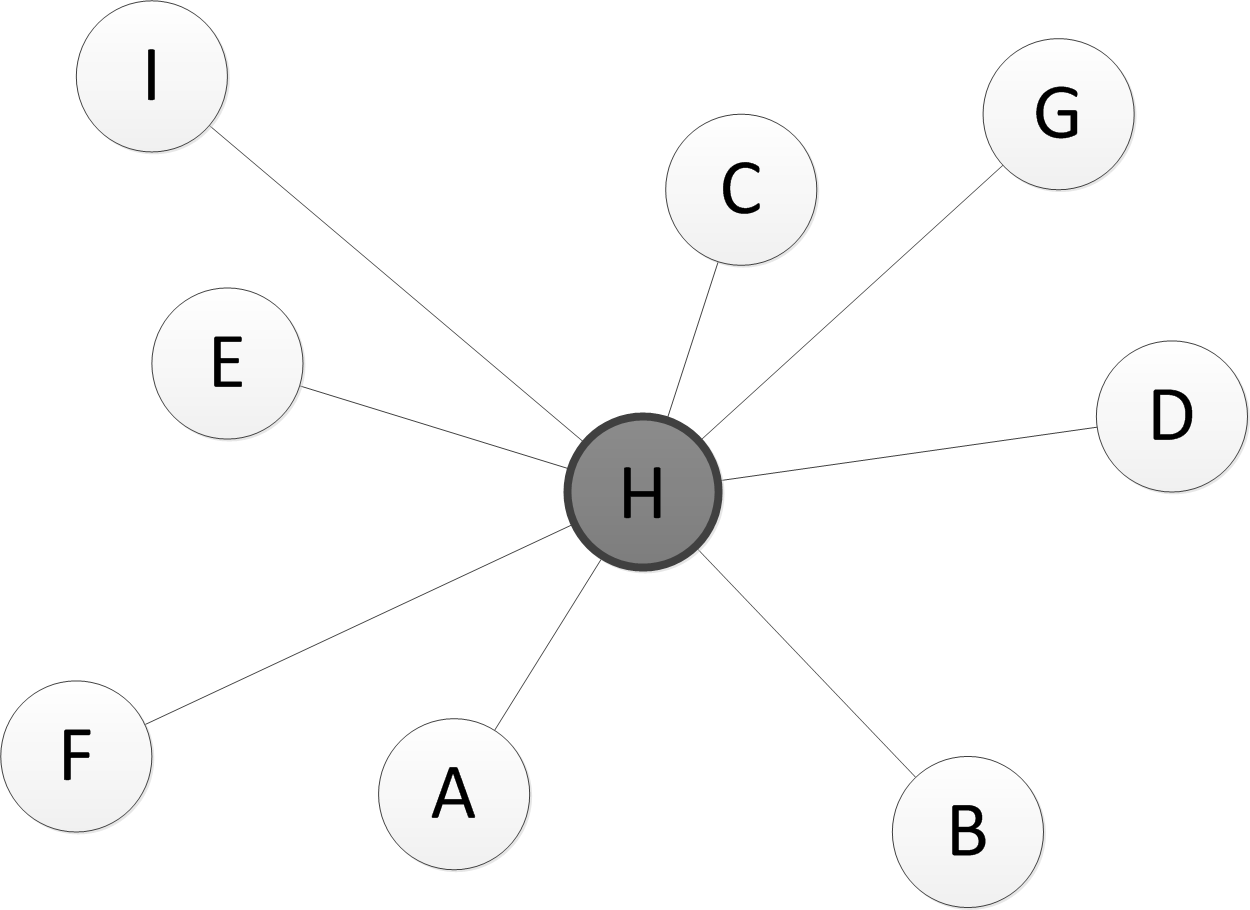
\includegraphics[scale=0.24]{hub_and_spoke_model.png} }
	\caption{Model "Hub and spoke"}\label{fig:hub_and_spoke}
\end{figure}

Rozwiązania oparte na serwerach aplikacji upraszczają impementacje komunikacji ponieważ serwery te zazwyczaj są wyposażone w obsługę standardowych protokołów takich jak HTTP czy SOAP. Minusem tych rozwiązań jest to, że logika integracyjna i logika biznesowa przeplatają sie nawzajem, a także poszczególne części systemu są dość mocno ze sobą powiązane co zmniejsza elastyczność systemu.

EAI brokers wypadają lepiej od serwerów aplikacji ponieważ rozdzielają logike integracyjną od logiki biznesowej. Jednak rozwiązanie to posiada wszystkie wady związane z modelem hub and spoke na którym jest oparte.

Rozwiązania bazujące na MOM pozwalają na luźne łączenie poszczególnych systemów a także na asynchroniczną komunikację między nimi. Rozwiązania te zazwyczaj nie posiadają wysoko poziomowej warstwy abstrakcji nad logiką routowania co fragmentami wymusza programowanie na dość niskim poziomie. Z tego też powódu, rozwiązania te, podobnie jak rozwiązania oparte na serwerach aplikacji cierpią z powodu przeplatającecj sie logiki integracyjnej z logiką biznesową, co utrudnia utrzymywanie i rozwijanie takiego systemu.

Ostatnia grupa rozwiązań jest oparta na ESB. Jest to zdecydowanie najnowsza z wyżej opisanych technologii. Dzięki doświadczeniu zdobytemu przy użytkowaniu poprzedników, udało sie stworzyć technologię, która nie posiada tych samych wad. Ogólnie rzecz ujmując ESB dostarcza warstwę abstrakcji opartą na implementacji biznesowego systemu wymiany wiadomości, dzięki temu pozwala wykorzystać zalety wiadomości bez pisania dodatkowego kodu. W przeciwieństwie do bardziej klasycznego podejścia (EAI) opartego o architekturę hub and spoke podstawa paltformy jest zbudowana z funkcji bazowych podzielonych na części składowe które mogą być osadzane zarówno w jednolitym jak i rozproszonym środowisku wzajemnie ze sobą współpracując. Szkielet ESB do zarządzania serwisami wykorzystuje komunikację działającą w oparciu o asynchroniczne przesyłanie wiadomości, ten sam system jest wykorzystywany do komunikacji pomiędzy serwisami osadzonymi w kontenerze. Najważniejszą cechą ESB jest fakt, iż po wpięciu aplikacji przez ściśle zdefiniowany, bazujący na standardach interfejs, uzyskuje ona dostęp do całej infrastruktury i serwisów udostpępnianych przez ESB a także do każdej innej, już działającej aplikacji. W chwili obecnej dostępnych jest kilka różnych implementacji ESB, większość z nich udostępnia podobne serwisy więc ciężko je stosować jako kryterium, lepszym sposobem by rozróżnić implementacje jest zastosowanie następującej miary:
\begin{itemize}
	\item wspierane środowisko działania/osadzania
	\item model kontenera - bazujący na standardach czy własnościowy
	\item powiązanie z innymi elementami architektury
	\item zależności
\end{itemize}

\setlength\fboxsep{20pt}
\setlength\fboxrule{1pt}
\begin{figure}[!h]
	\centering
	\fbox{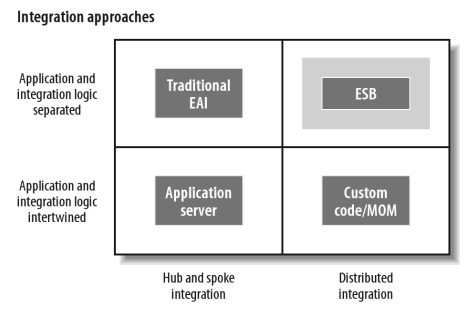
\includegraphics{podejscia_integracyjne.png} }
	\caption{Różne podejścia integracyjne  \cite{chappell2004}}\label{fig:podejscia_integracyjne}
\end{figure}

\newpage

\section{Inegracja systemów przetwarzania mowy}

Podrozdział ten ma na celu przedstawić jakie wymagania można postawić przed przykładową aplikacją integrującą systemy przetwarzania mowy i jak wpłyną one na sposób integracji. Aby zdefiniować wymagania można rozważyć przykładową aplikację kliencką która mogłaby być zbudowana w oparciu o taki system. Podstawowe funkcje które taka aplikacja realizuje mogą być następujące:
\begin{itemize}
	\item zamiana pliku graficznego będącego zdjęciem tekstu na plik tekstowy
	\item synteza tekstu
	\item tłumaczenie tekstu
	\item rozpoznanie języka tekstu
	\item zamiana mowy na tekst
\end{itemize}
Oczywiście każde z wyżej wymienionych zadań może zostać zrealizowane osobno przez odpowiednie aplikacje. Dlatego, gotowy system powinien być w stanie realizować każdą z nich osobna jak i każdą możliwą i sensowną kombinację. Dobrym przykładem takiej złożonej funkcjonalności jest zamiana pliku w formacie graficznym, będącym zdjęciem np. strony ksiązki(napisanej w nieznanym języku) na dźwięk w jakimś innym, konkretnym, zdefiniowanym przez użytkownika języku. Aby to osiągnąć należy poinformować system o tym z których serwisów należy skorzystać i w jakiej koleności je wywołać. Oczywiście idealnym i na szczeście możliwym rozwiązaniem jest ukrycie całej implementacji za jednym prostym interfersjem. Proponowanym rozwiązaniem tego problemu jest plik sterujący w formacie XML. Przykładowa struktura takiego pliku mogłaby wyglądać następująco:
 \begin{itemize}
	\item \textless speechProcessingInstructions\textgreater - podstawowy element, będący korzeniem dla całego pliku
	\item \textless readImage\textgreater - wystąpienie tego elementu oznacza, że na wejściu należy oczekiwać pliku graficznego, zawierającego tekst
	\item \textless identifyLanguage\textgreater - element oznaczający konieczność użycia serwisu rozpoznającego język
	\item \textless translate\textgreater - element wymuszający użycie translatora, jego dziećmi są następujące elementy:
		 \begin{itemize}
			\item \textless inputLanguage\textgreater - element, którego zastosowaniem jest zdefiniowane języka tekstu wejściowego, jeżeli operacją poprzednią  było rozpoznanie języka element ten zostanie pominięty
			\item \textless outputLanguage\textgreater - element, którego zastosowaniem jest zdefiniowane języka tekstu docelowego
		\end{itemize}
	\item \textless performTTS\textgreater - element oznaczający konieczność wywołania serwisu odpowiadającego za syntezę mowy
	\item \textless performASR\textgreater - wystąpienie tego elementu oznacza użycie serwisu odpowiedzialnego  za rozpoznawanie mowy
\end{itemize}
Zastosowanie takiego formatu ma dużo zalet, z czego najważniejsze to:
\begin{itemize}
	\item prostota
	\item duża ilość narzędzi do pracy z XML
	\item wysoki poziom zadomowienia tego formatu w środowisku SOA
	\item czytelność dla człowieka
	\item łatwa rozbudowa
\end{itemize}
Aby zrealizować opisany wyżej scenariusz należałoby wysłać następujący plik XML:

\setlength\fboxsep{20pt}
\setlength\fboxrule{1pt}
\begin{figure}[!h]
	\centering
	\fbox{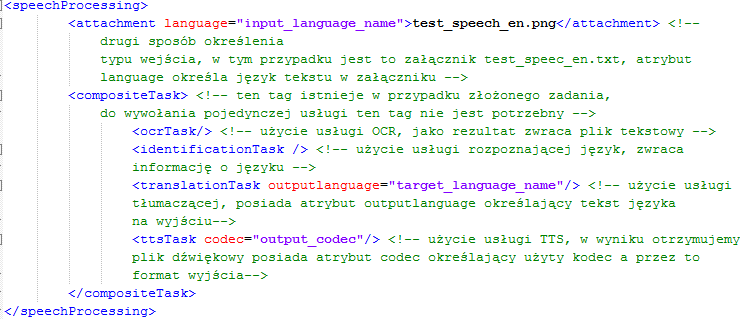
\includegraphics[scale=0.8]{sampleXML.png} }
	\caption{Przykładowy plik XML}
\end{figure}

Podsumowując, zakładając istnienie tak działającego systemu, jedyne zadania jakie musiałaby spełniać aplikacja kliencka:
\begin{itemize}
	\item umożliwić użytkownikowi łatwe wygenerowanie pliku sterującego XML
	\item opcjonalne (zależnie od scenariusza) pobranie pliku graficznego lub tekstowego i przesłanie go do systemu
	\item pobranie strumienia dźwięku i przesłanie go do systemu
	\item przekazać użytkownikowi rezultat działania systemu (np. plik z przetlumaczonym tekstem, plik dźwiękowy, strumień dzwięku itd.)
\end{itemize}
Jak widać są to rzeczy dość proste i możliwe do bardzo szybkiej implementacji. Oczywiście bardzo łatwo można wyobrazić sobie możliwości rozbudowy takiej platformy. Jednym z kierunków takiej rozbudowy może być chęć wykorzystania innych, niż opisane wyżej(plik graficzny, plik xml) formatów danych wejściowych.  Bardzo pomocne okażą się tutaj endpoint'y, oferowane przez niemal każdą implementację ESB, umożliwiające łatwe pobieranie danych z różnych źródeł, takich jak:
\begin{itemize}
	\item mail
	\item ftp
	\item serwisy webowe
	\item RSS
	\item serwisy REST'owe
\end{itemize}
Łatwo wyobrazić sobie użycie endpointów, można je na przykład wykorzystać aby umożliwić użytkownikowi dostęp do serwisu drogą mailową. Wystarczy aby użytkownik wysłał na specjalny adres maila zawierającego, w postaci załączników, plik sterujący xml oraz plik wejściowy, na przykład zdjęcie tekstu albo tekst, w efekcie czego otrzymałby maila zwrotnego z danymi uzyskanymi w wyniku wykonania żądanych przez niego operacji. Innym przykładem użycia endpointów, w celu zwiększenia funkcjonalności systemu, mogłoby być rozbudowanie pliku sterującego na przykład o tag \textless rssSource\textgreater który sprawi, że aplikacja zamiast pliku wejściowego pobierze wiadomości ze źródła RSS i na nich wywoła funkcje udostępniane przez serwisy. Jak widać wykorzystanie endpoint'ów daje wiele możliwości i idealnie wkomponowuje się w dziedzinę problemu, co stanowi kolejny argument na rzecz wykorzystania ESB jako sposobu integracji.

\section*{Podsumowanie}
Biorąc pod uwagę proponowane serwisy, format danych wejściowych i wymagania stawiane przed platformą zdecydowanie najlepszym sposobem integracji wydaje się wykorzystanie jednej z istniejących implementacji ESB. Wszystkie one zapewniają routing, dużo różnych endpointów, wsparcie dla aplikacji pisanych przy użyciu Springa i wiele innych rzeczy które można wykorzystać nie tylko przy implementacji podsatawowej wersji systemu ale także przy jego rozbudowie. 



%ksiazka ESB strony 4,5 

%opiszemy to podejscie i potem opiszemy, ze jest bardzo fajne, opiszemy rodzaje, jak ewoluowało, i na koncu opiszemy esb, a potem konkrety dla naszej aplikacji. Obrazki w ksiazce ESB
%ESB strona 34 - czemu własnościowe rozwiązania sa do dupy 



%\subsection {Szyna} 

%Przedstawienie jak to wyglada( kropki serwisy , komunikują sie z roznymi innymi serwisami, dodatokwe serisy: accounting itd)

%Wymagania stawiane rozwiazaniom integracyjnym , Czy warto integrować ? (book1.pdf chapter 2)

%Integracja systemow multimedialnych ??

%Rozwiazania ?

%Brak integracji

%integracja EAI - hub and spikes (scentralizowany punk, single point of failure. słabo scalowalne)

%SOA - ESB 




%service activator (request od clienta)


% ---------------------------------------------------------------------------
%: ----------------------- end of thesis sub-document ------------------------
% ---------------------------------------------------------------------------

